\documentclass{beamer}
\usepackage[utf8]{inputenc}
\usepackage[graphicx]

\author[Sowmya Vajjala]{Instructor: Sowmya Vajjala}


\title[LING 120]{Language and Computers}
\subtitle{Semester: FALL '17}

\date{27 October 2017}

\institute{Iowa State University, USA}

%%%%%%%%%%%%%%%%%%%%%%%%%%%

\begin{document}

\begin{frame}\titlepage
\end{frame}

\begin{frame}
\frametitle{Outline}
\begin{enumerate}
\item Dialog systems: Introduction
\item Plan: Monday - How dialog systems are designed. Wednesday - How are they evaluated?
\item Upcoming deadlines: Assignment 5, Next week!
\end{enumerate}
\end{frame}
%Class full of questions on dialogue systems?

\begin{frame}
\frametitle{Startup questions}
\begin{enumerate}
\item What do these terms dialog systems or conversational agents/bots mean to you? \pause
\item Why do you think they are useful in real world? \pause
\item Did you use any conversational bot or mobile-phone assistants? \pause
\item If you used, what is your general impression? \pause
\item What challenges do you see in the development of such computer systems? \pause
\item Do you think eventually they should resemble conversations with humans? \pause
\item If so, how should these dialog systems be designed? 
\end{enumerate}
\end{frame}

\begin{frame}
\frametitle{General principles of human communication}
\begin{enumerate}
\item The speaker initiates a conversation after thinking about what to say, what is the purpose, and how to communicate. 
\item The listener has to notice this, understand both literal and contextual meaning of what was said, and the intent.
\item The listener will then formulate a response, also ensuring that general social conventions and niceties are in place. \pause
\item Humanbeings are highly skilled at this since young age. We are so good we dont even notice how we do.
\item You saw with Eliza example this need not be the case for computers. \pause
\end{enumerate}
\end{frame}

\begin{frame}
\frametitle{Insights from Pragmatics-1}
\framesubtitle{Organization of a conversation}
\begin{enumerate}
\item Pragmatics is a sub-field of linguistics concerned about conversations, and how context contributes to meaning.
\item They describe human dialogs in terms of "moves":
\begin{itemize}
\item Initiating moves - making a request, asking a question, issuing a command, making a general statement etc.
\item Response moves - saying yes/no, giving longer response, conditional/partial agreement etc
\item Dialog management moves - clarification questions, general nods, exclamations, saying "i take it back" etc.
\end{itemize}
\end{enumerate}
Question: How does understanding these make sense for a dialog system? 
\end{frame}

\begin{frame}
\frametitle{Insights from Pragmatics-2}
\framesubtitle{What individual utterances in a dialog do}
\begin{enumerate}
\item Informing, Reminding, Commanding, Refusing, Accepting etc.
\item Talk directly or indirectly
\item This is studied in detail under the heading "Speech Acts" in Pragmatics
\end{enumerate}
Same question: How does understanding these make sense for a dialog system? 
\end{frame}

\begin{frame}
\frametitle{Insights from Pragmatics-3}
\framesubtitle{Rules of Conversation - Gricean Maxims}
(Proposed by H.P.Grice in 70s)
\begin{enumerate}
\item Maxim of quality:  Give correct information.
\item Maxim of quantity: Do not over-talk
\item Maxim of relation: Be relevant.
\item Maxim of manner: avoid ambiguity, being "orderly" etc
\end{enumerate}
Details: \url{https://en.wikipedia.org/wiki/Cooperative_principle}
\end{frame}

\begin{frame}
\frametitle{Applying these insights in dialog system design}
\begin{itemize}
\item Broadly speaking, there are two kinds of dialog systems - task oriented, and chat bots.
\item Task oriented: designed for specific tasks, and to have short, specific conversations to get questions from user and collect answers. (Google Assistant, Siri, Flight booking systems etc)
\item Chat Bots: Extended casual, human-like conversations, with or without specific task focus (Eliza) \pause (both terms are used synonymously nowadays)
\item How to apply these insights from Pragmatics to dialog systems depends on the application scenario too. \pause
\item Let us take one task oriented dialog system - LetsGo from CMU which is actually being used in the public transit system in Pittsburgh. (the phone number did not work for me)
\\ \url{http://www.speech.cs.cmu.edu/letsgo/} (video and transcript)
\end{itemize}
\end{frame}

\begin{frame}
\frametitle{Another application domain for task-oriented systems: Tutoring systems}
\framesubtitle{Image source: Speech and Language Processing 3rd Edition}
One example: 
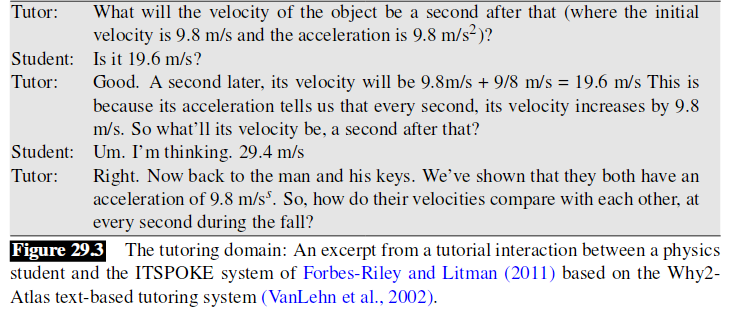
\includegraphics[width=0.9\textwidth]{tutoringdialog.png}
\\ \pause Another real world example: cognii virtual learning assistant (\url{https://www.youtube.com/watch?v=Jk_3Mk_QCGA})
\end{frame}

\begin{frame}
\frametitle{AI based Chat-bots}
\begin{itemize}
\item \url{https://morph.ai/demos}
\item \url{https://x.ai/}
\item Tools that support building your own intelligent bots:
\begin{enumerate}
\item \url{https://chatfuel.com/}
\item \url{https://dev.botframework.com/}
\end{enumerate}
\item Recent example: Woebot, a AI powered facebook bot that can help you with depression. 
\\ \url{https://www.woebot.io/}
\\ Relevant news article: \url{https://goo.gl/GyLjiH} \pause
\item "Natural Language Processing and Machine Learning: The core of the modern, smart chatbot."
\\ \url{https://goo.gl/bSTSNX}
\end{itemize}
\end{frame}

\begin{frame}
\frametitle{Continuously improving.. : Siri in 2014}
\framesubtitle{Image source: Speech and Language Processing 3rd Edition}
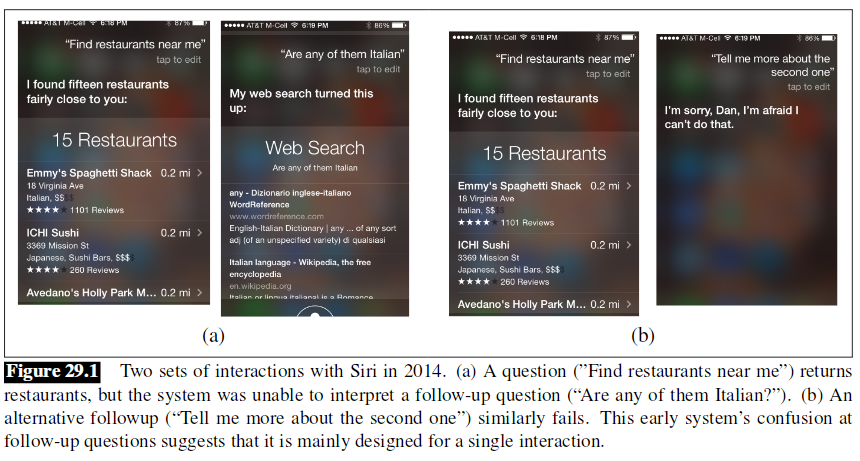
\includegraphics[width=0.9\textwidth]{siri2014.png}
\end{frame}

\begin{frame}
\frametitle{Continuously improving.. : Siri in 2017}
\framesubtitle{Image source: Speech and Language Processing 3rd Edition}
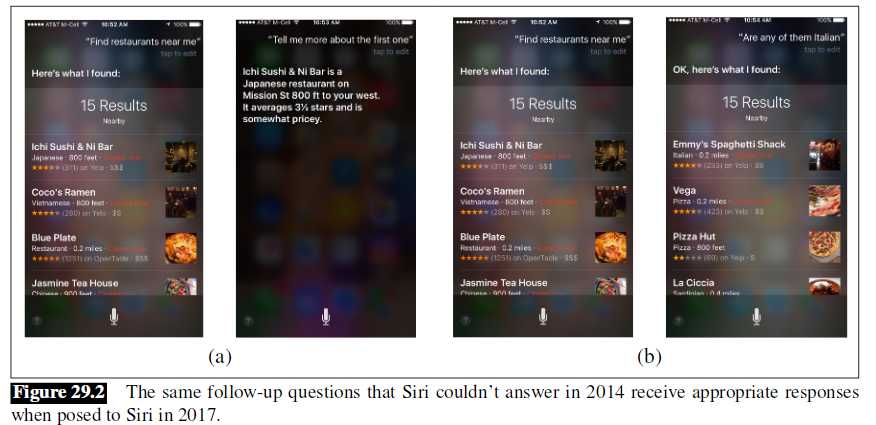
\includegraphics[width=0.9\textwidth]{siri2017.png}
\pause \\ This may sound impressive, but there is still some way to go. E.g., It could not identify Jack Trice in Indian accent: It identified as Jack Device, Jack Ties, Jack Twice, Jack Place but never as Jack Trice despite multiple trials.
\end{frame}

\begin{frame}
\frametitle{Siri: on 11 Jan and Today on my office machine}
\includegraphics[width=0.9\textwidth]{Siri-ThenNow.png}
\end{frame}

\begin{frame}
\frametitle{Speculations}
\begin{itemize}
\item Based on what you understand so far and what you saw with Eliza or Siri or something, what do you expect the dialog systems to do for you in current day?
\item After 5 years, how do you think this will look? \pause
\item After 20 years? \pause
\end{itemize}
\end{frame}

\begin{frame}
\frametitle{Attendance Exercise}
Here are a few conversations I had with Siri this morning. What do you is happening here? Where is it doing better? Where can it do better? (I am not asking how can I do better!)
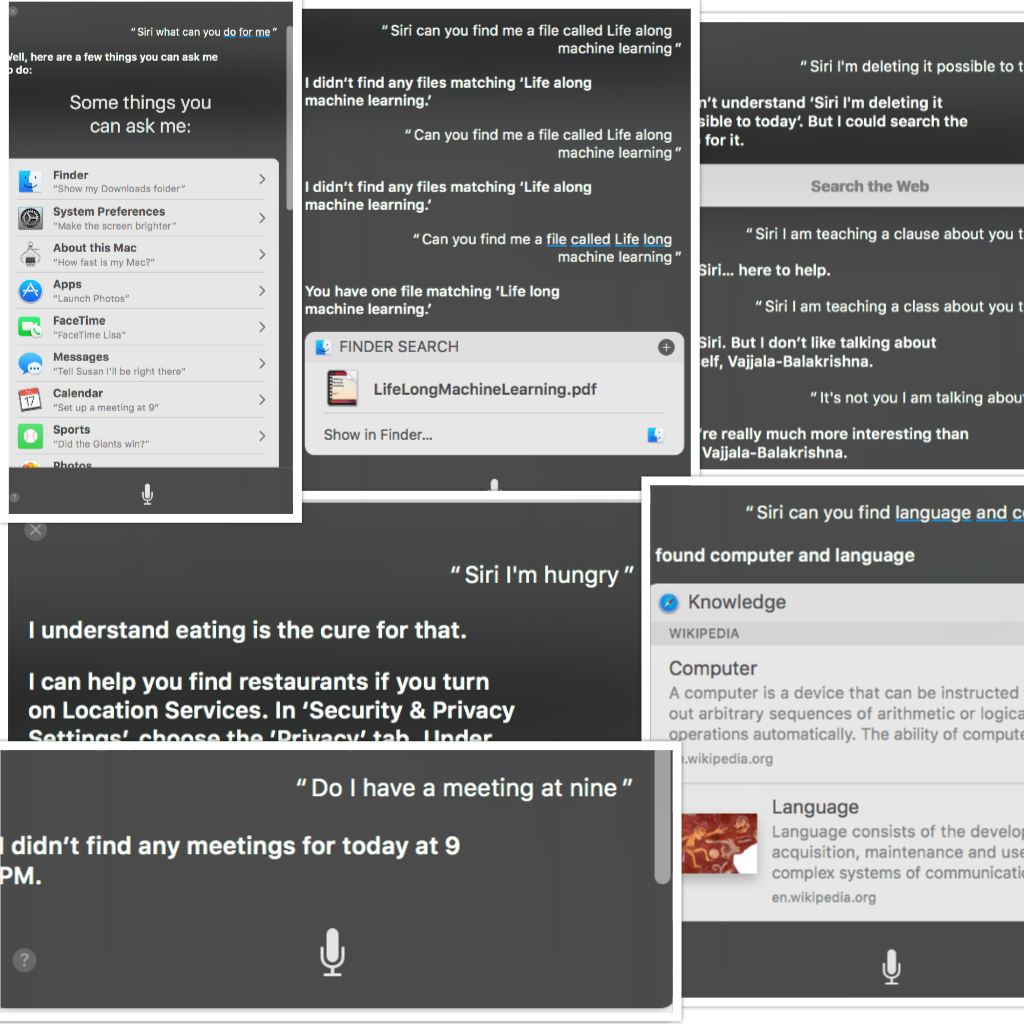
\includegraphics[width=0.6\textwidth]{collage-siri.png} 
\end{frame}

\begin{frame}
\frametitle{Next Week}
\begin{itemize}
\item Deadlines: Assignment 5 submission deadline.
\item Topics: Dialog Systems - design and evaluation, Introduction to Speech recognition
\item Readings: Chapter 6 in the textbook (Especially the "Under the Hood" section on how Eliza works)
\item I will get back to your responses about Eliza next week.
\end{itemize}
\end{frame}

\end{document}

%MONDAY: %Major ways of writing chatbots: J&M - Rules, IR and Transduction models
%Eliza, Airport flight booking, and FAQ bot examples

%For wednesday: http://www.wildml.com/2016/04/deep-learning-for-chatbots-part-1-introduction/#more-750
